\documentclass[10pt, a4paper, titlepage]{article}

% ---
% --- Formatting
\usepackage[portrait, margin=0.8cm]{geometry}
\usepackage{caption}
\usepackage{float}
\usepackage[none]{hyphenat}
\usepackage{multicol}
\usepackage{sectsty}
\usepackage{subcaption}

% Removes heading numbers of headers. Disable for numbers and to create a table of contents.
\setcounter{secnumdepth}{0}

% Makes headers and footers empty: removes page numbers
\pagestyle{empty}

% Line between columns
%\setlength{\columnseprule}{0.4pt}

%\setlength{\parskip}{1em}

% Disables paragraph indents
\setlength{\parindent}{0em}

% Toggle column vertical alignment
\raggedcolumns


% ---
% --- Typography
\usepackage[utf8]{inputenc}

% Sets heading font sizes.
\sectionfont{\large}
\subsectionfont{\normalsize}

% ---
% --- Graphics
\usepackage{graphicx}
\graphicspath{{images/}}


% ---
% --- Math
\usepackage{amsmath}
\usepackage{amssymb}
\usepackage{physics}

% Removes equation label numbers
\makeatletter
\renewcommand\tagform@[1]{}
\makeatother

\DeclareMathOperator\cis{cis}


\begin{document}

\title{12 Specialist Mathematics Summarised Notes \\ (Unofficial) \\ Work in Progress}
\author{}
\date{}
\maketitle

% Content begins below
\begin{multicols*}{3}

\section{Functions}
	\subsection{Composite Functions}
	Given $f:x\mapsto f(x)$ and $g:x\mapsto g(x)$, the composite function of $f$ and $g$ is:
	\begin{gather}
		(f\circ g)(x)=f(g(x))\\
		\text{or}\\
		f\circ g:x\mapsto f(g(x))
	\end{gather}
	In general, $(f\circ g)(x)\neq (g\circ f)(x)$.

	\dotfill
	\subsection{Inverse Functions}
	An inverse function returns the original value from the output of a function.\\
	$f(x)$ has an inverse if it is injective (one-to-one), if $f(a)=f(b)$ only when $a=b$, $\therefore$ passes the horizontal line test.\\\\
	For $f^{-1}(x)$, the inverse of $f(x)$:
	\begin{itemize}
		\item Is a reflection of $y=f(x)$ over $y=x$.
		\item $(f\circ f^{-1})(x)=(f^{-1}\circ f)(x)=x$
		\item Domain of $f^{-1}=$ range of $f$.
		\item Range of $f^{-1}=$ domain of $f$.
	\end{itemize}

	\dotfill
	\subsection{Self-Inverse Functions}
	An invertible function that is symmetrical about $y=x$.
	\begin{align}
		f^{-1}(x)=f(x)
	\end{align}

	\dotfill
	\subsection{Reciprocal Functions}
	A function of the form $f(x)=\cfrac{k}{x}$, where $k\neq 0$ is a constant.

	\dotfill
	\subsection{Reciprocal of Other Functions}
	The reciprocal of a function $f(x)$ is $\frac{1}{f(x)}$.\\
	\underline{Graphing $y=\frac{1}{f(x)}$ from $y=f(x)$:}
	\begin{itemize}
		\item Zero $f(x)\to$ vertical asymp $\frac{1}{f(x)}$
		\item Vertical asymp $f(x)\to$ zero $\frac{1}{f(x)}$
		\item Local max $f(x)\to$ local min $\frac{1}{f(x)}$
		\item Local min $f(x)\to$ local max $\frac{1}{f(x)}$
		\item When $f(x)>0,\ \frac{1}{f(x)}>0$
		\item When $f(x)<0,\ \frac{1}{f(x)}<0$
		\item When $f(x)\to 0,\ \frac{1}{f(x)}\to \pm \infty$
		\item When $f(x)\to \pm \infty,\ \frac{1}{f(x)}\to 0$
	\end{itemize}
	\underline{Invariant Points:}
	\\Points that do not move under a transformation occurring at $y=\pm 1$.

	\dotfill
	\subsection{Rational Functions}
	Results from the division of one polynomial by another.\\
	Vertical asymptote occurs when denominator is zero.\\
	Horizontal asymptote ascertained from behaviour of graph as $|x|\to \infty$.
	\begin{itemize}
		\item If the degree of denominator $>$ numerator, horizontal asymptote at $y=0$.
		\item If the degree of denominator $<$ numerator, function has slanted asymptote found through polynomial division.
		\item If the degree of denominator $=$ numerator horizontal asymptote at $y=\frac{a}{b}$ where $a$ and $b$ are the leading coefficients.
	\end{itemize}

	\dotfill
	\subsection{Absolute Value Functions}
	The absolute value or modulus $|x|$ of a real number $x$ is its distance from 0 on the number line.
	\begin{align}
		|x|=
		\begin{cases}
			x\,&\text{if } x\geq 0\\
			-x\,&\text{if } x < 0 
		\end{cases}
	\end{align}
	Alternatively,
	\begin{align}
		|x|=\sqrt{x^2}
	\end{align}
	\underline{Properties:}
	%\begin{align}
	%	&|x|\geq0&& &&|-x|=|x|&\\
	%	&|x|^2=x^2&& &&|xy|=|x||y|&\\
	%	&\left|\frac{x}{y}\right|=\frac{|x|}{|y|}&& &&|x-y|=|y-x|&\\
	%\end{align}
	\begin{itemize}
		\item $|x|\geq0$
		\item $|x|^2=x^2$
		\item $\left|\frac{x}{y}\right|=\frac{\left|x\right|}{\left|y\right|}$
		\item $|-x|=|x|$
		\item $|xy|=|x||y|$
		\item $|x-y|=|y-x|$
	\end{itemize}
	If $|x|=a$ where $a>0$, then $x=\pm a$.\\
	If $|x|=|b|$ then $x=\pm b$.

	\dotfill
	\subsection{Graphs Involving the Absolute Value Function}
	\underline{Graphing $y=f(|x|)$ from $y=f(x)$:}
	\begin{itemize}
		\item Discard the graph for $x<0$
		\item Reflect the graph for $x\geq 0$ in the $y$-axis
		\item Points on the $y$-axis are invariant
	\end{itemize}
	\underline{Graphing $y=|f(x)|$ from $y=f(x)$:}
	\begin{itemize}
		\item Keep the graph for $f(x)\geq 0$
		\item Reflect the graph for $f(x)<0$ in the $x$-axis
		\item Points on the $x$-axis are invariant
	\end{itemize}
	\hrulefill


\section{Trigonometric Identities}
	\subsection{Angle Relationships}
	%\begin{align}
	%	&\sin{(-\theta)}=-\sin{\theta}&& &&\cos{(-\theta)}=\cos{\theta}&\\
	%	&\sin{(\pi -\theta)}=\sin{\theta}&& &&\cos{(\pi -\theta)}=-\cos{\theta}&\\
	%	&\sin{\left(\frac{\pi}{2}-\theta \right)}=\cos{\theta}&& &&\cos{\left(\frac{\pi}{2}-\theta \right)}=\sin{\theta}&
	%\end{align}
	\resizebox{.9\linewidth}{!}{
		\begin{minipage}{\linewidth}
			\begin{align}
				&\sin{(-\theta)}=-\sin{\theta}&& &&\cos{(-\theta)}=\cos{\theta}&\\
				&\sin{(\pi -\theta)}=\sin{\theta}&& &&\cos{(\pi -\theta)}=-\cos{\theta}&\\
				&\sin{\left(\frac{\pi}{2}-\theta \right)}=\cos{\theta}&& &&\cos{\left(\frac{\pi}{2}-\theta \right)}=\sin{\theta}&
			\end{align}
		\end{minipage}
	}\\

	%\begin{flalign}
	%	&\quad \sin{(-\theta)}=-\sin{\theta}&&\\
	%	&\quad \cos{(-\theta)}=\cos{\theta}&&\\
	%	&\quad \sin{(\pi -\theta)}=\sin{\theta}&&\\
	%	&\quad \cos{(\pi -\theta)}=-\cos{\theta}&&\\
	%	&\quad \sin{\left(\frac{\pi}{2}-\theta \right)}=\cos{\theta}&&\\
	%	&\quad \cos{\left(\frac{\pi}{2}-\theta \right)}=\sin{\theta}&&
	%\end{flalign}

	\dotfill
	\subsection{Pythagorean Theorem}
	\begin{flalign}
		&\quad \sin^2{\theta}+\cos^2{\theta}=1&&\\
		&\quad \tan^2{\theta}+1=\sec^2{\theta}&&\\
		&\quad \cot^2{\theta}+1=\csc^2{\theta}&&
	\end{flalign}

	\dotfill
	\subsection{Double Angle Identities}
	\begin{flalign}
		\quad \sin{2\theta}&=2\sin{\theta}\cos{\theta}&&\\
		\quad \cos{2\theta}&=\cos^2{\theta}-\sin^2{\theta}&&\\
		&=1-2\sin^2{\theta}&&\\
		&=2\cos^2{\theta}-1&&\\
		\quad \tan{2\theta}&=\frac{2\tan{\theta}}{1-\tan^2{\theta}}&&
	\end{flalign}

	\dotfill
	\subsection{Angle Sum and Difference}
	\begin{flalign}
		&\quad \sin{(A\pm B)}=\sin{A}\cos{B}\pm \cos{A}\sin{B}&&\\
		&\quad \cos{(A\pm B)}=\cos{A}\cos{B}\mp \sin{A}\sin{B}&&\\
		&\quad \tan{(A\pm B)}=\frac{\tan{A}\pm \tan{B}}{1\mp \tan{A}\tan{B}}&&
	\end{flalign}

	\dotfill
	\subsection{Sum to Product}
	\resizebox{.85\linewidth}{!}{
		\begin{minipage}{\linewidth}
			\begin{flalign}
				&\quad \sin{A}\pm \sin{B}=2\sin{\left(\frac{A\pm B}{2}\right)}\cos{\left(\frac{A\mp B}{2}\right)}&&\\
				&\quad \cos{A}+\cos{B}=2\cos{\left(\frac{A+B}{2}\right)}\cos{\left(\frac{A-B}{2}\right)}&&\\
				&\quad \cos{A}-\cos{B}=-2\sin{\left(\frac{A+B}{2}\right)}\sin{\left(\frac{A-B}{2}\right)}&&
			\end{flalign}
		\end{minipage}
	}\\

	\dotfill
	\subsection{Product to Sum}
	\resizebox{.93\linewidth}{!}{
		\begin{minipage}{\linewidth}
			\begin{flalign}
				&\quad 2\sin{A}\cos{B}=\sin{(A+B)}+\sin{(A-B)}&&\\
				&\quad 2\sin{A}\sin{B}=\cos{(A-B)}-\cos{(A+B)}&&\\
				&\quad 2\cos{A}\cos{B}=\cos{(A+B)}+\cos{(A-B)}&&
			\end{flalign}
		\end{minipage}
	}\\

	\hrulefill


\section{Mathematical Induction}
	\subsection{The Principle of Mathematical Induction}
	Suppose $P_n$ is a proposition which is defined for every integer $n\geq a$, $a\in \mathbb{Z}$. If $P_a$ is true, and if $P_{k+1}$ is true whenever $P_k$ is true, then $P_n$ is true for all $n\geq a$.

	\hrulefill


\section{Complex Numbers}
	\subsection{Imaginary Numbers}
	A number which cannot be placed on a real number line in the form $ai$ where $a\in \mathbb{R}$ and $i=\sqrt{-1}$.\\

	\dotfill
	\subsection{Complex Numbers}
	Any number in the form $a+bi$ where $a,b\in \mathbb{R}$ and $i=\sqrt{-1}$.
	\begin{gather}
		\begin{flalign}
			&\text{If}\quad z=a+bi&&
		\end{flalign}\\
		\mathfrak{Re} (z)=a\qquad \mathfrak{Im} (z)=b
	\end{gather}

	\dotfill
	\subsection{The Complex Plane}
	Complex numbers can be plotted on the complex plane or Argand plane as a vector where the $x$-axis is the real axis and the $y$-axis is the imaginary axis.
	\begin{align}
		\overrightarrow{OP}=\begin{pmatrix}x\\ y\end{pmatrix}\quad \text{represents}\quad x+yi
	\end{align}
	\dotfill
	\subsection{Complex Conjugates}
	The complex conjugate of
	\begin{align}
		z=a+bi\qquad \text{is}\qquad z^*=a-bi
	\end{align}
	In the complex plane, $z^*$ is the reflection of $z$ in the real axis.

	\dotfill
	\subsection{Modulus and Argument}
	The modulus of the complex number \\$z=a+bi$ is the length of the vector $\big(\begin{smallmatrix}a\\ b\end{smallmatrix}\big)$, which is the real number:
	\begin{align}
		|z|=\sqrt{a^2+b^2}
	\end{align}
	The argument of $z$, $\arg({z})$ is the angle $\theta$ between the positive real axis and $\big(\begin{smallmatrix}a\\ b\end{smallmatrix}\big)$.\\
	Real numbers have an argument of 0 or $\pi$.\\
	Purely imaginary numbers have argument of $\frac{\pi}{2}$ or $-\frac{\pi}{2}$.\\

	\underline{Properties of Modulus:}
	\begin{itemize}
		\item $|z^*|=|z|$
		\item $|z^*|^2=zz^*$
		\item $|z_1z_2|=|z_1||z_2|$
		\item $\left|\frac{z_1}{z_2}\right|=\frac{|z_1|}{|z_2|},\ z_2\neq 0$
		\item $|z_1z_2z_3\dots z_n|=|z_1||z_2||z_3|\dots |z_n|$
		\item $|z^n|=|z|^n,\ n\in \mathbb{Z}^+$
	\end{itemize}

	\dotfill
	\subsection{Polar Form}
	%\begin{gather}
	%	\cis{\theta}=\cos{\theta}+i\sin{\theta}\\
	%	\begin{flalign}
	%		&\text{A complex number $z$ has polar form}&&
	%	\end{flalign}\\
	%	z=|z|\cis{\theta}\\
	%	\begin{flalign}
	%		&\text{where $\theta = \arg{z}$.}&&\\
	%		&\text{The conjugate of $z$ is:}&&
	%	\end{flalign}\\
	%	z^*=|z|\cis{-\theta}
	%\end{gather}\\
	\begin{align}
		\cis{\theta}=\cos{\theta}+i\sin{\theta}
	\end{align}
	A complex number $z$ has the polar form
	\begin{align}
		z=|z|\cis{\theta}
	\end{align}
	where $\theta = \arg({z})$.\\
	The conjugate of $z$ is:
	\begin{align}
		z^*=|z|\cis{(-\theta)}
	\end{align}
	\underline{Properties of $\cis{\theta}$:}
	\begin{itemize}
		\item $\cis{\theta}\times \cis{\phi}=\cis{(\theta +\phi )}$
		\item $\frac{\cis{\theta}}{\cis{\phi}}=\cis{(\theta -\phi )}$
		\item $\cis{(\theta -2k\pi )}=\cis{\theta},\ k\in \mathbb{Z}$
	\end{itemize}

	% NOTE: Not in the course
	%\dotfill
	%\subsection{Euler's Form}
	%\begin{align}
	%	e^{i\theta}=\cos{\theta}+i\sin{\theta}
	%\end{align}

	\dotfill
	\subsection{De Moivre's Theorem}
	\begin{align}
		(|z|\cis{\theta})^n=|z|^n\cis{n\theta},\ \text{for all }n\in \mathbb{Q}
	\end{align}
	\dotfill
	\subsection{Roots of Complex Numbers}
	The $n^{\text{th}}$ roots of the complex number $c$ are the solutions of $z^n=c$.

	\dotfill
	\subsection{The $n^{\text{th}}$ Roots of Unity}
	The $n^{\text{th}}$ roots of unity are the solutions of $z^n = 1$.
	
	\dotfill
	\subsection{Distances in the Complex Plane}
	If $z_1\equiv \overrightarrow{OP_1}$ and $z_2\equiv \overrightarrow{OP_2}$ then $|z_1-z_2|$ is the distance between points $P_1$ and $P_2$.

	\hrulefill

\section{Real Polynomials}
	\subsection{Zeros and Roots}
	A zero of a polynomial is a value of the variable which makes the polynomial equal to zero.\\
	$\alpha$ is a zero of polynomial
	\begin{align}
		P(x)\iff P(\alpha)=0
	\end{align}
	The roots of a polynomial equation are the solutions to the equation.\\
	$\alpha$ is a root (or solution) of
	\begin{align}
		P(x)\iff P(\alpha)=0
	\end{align}
	The roots of $P(x)=0$ are the zeros of $P(x)$ and the $x$-intercepts of the graph $y=P(x)$
	
	\dotfill
	\subsection{Factors}
	$(x-\alpha)$ is a factor of the polynomial $P(x)\iff$ there exists a polynomial $Q(x)$ such that $P(x)=(x-\alpha)Q(x)$.
	
	\dotfill
	\subsection{Polynomial Equality}
	Two polynomials are equal if and only if they have the same degree (order) and corresponding terms have equal coefficients.
	
	\dotfill
	\subsection{Polynomial Division by Linears}
	If $P(x)$ is divided by $D(x)=ax+b$ until a quotient $Q(x)$ and constant remainder $R$ is obtained, then
	\begin{align}
		\frac{P(x)}{ax+b}=Q(x)+\frac{R}{ax+b}
	\end{align}
	Notice that $P(x)=Q(x)\times (ax+b)+R$.
	
	\dotfill
	\subsection{Polynomial Division by Quadratics}
	If $P(x)$ is divided by $D(x)=ax^2+bx+c$, then
	\begin{align}
		\frac{P(x)}{ax^2+bx+c}=Q(x)+\frac{ex+f}{ax^2+bx+c}
	\end{align}
	where $ex+f$ is the remainder.
	
	\dotfill
	\subsection{The Remainder Theorem}
	When a polynomial $P(x)$ is divided by $x-k$ until a constant remainder $R$ is obtained, then $R=P(k)$.
	
	\dotfill
	\subsection{The Factor Theorem}
	For any polynomial $P(x)$, $k$ is a zero of $P(x)\iff (x-k)$ is a factor of $P(x)$.
	
	\dotfill
	\subsection{The Fundamental Theorem of Algebra}
	If $P(x)$ is a polynomial of degree $n$, then $P(x)$ has $n$ zeros, each in the form $a+bi$ where $a,b\in \mathbb{R}$, some of which may be repeated.
	
	% TODO: Things not in the course can be highlighted in red to indicate extra content
	% NOTE: Not in the course

	%\dotfill
	%\subsection{Sum and Product of Roots}
	%For the polynomial equation
	%\begin{gather}
	%	\sum_{r=0}^{n}a_rx^r=0,\quad a_n\neq 0\\
	%	\begin{align}
	%		\text{Sum of roots: }&\frac{-a_{n-1}}{a_n}\\
	%		\text{Product of roots: }&\frac{(-1)^na_0}{a_n}
	%	\end{align}	
	%\end{gather}
	\hrulefill

\section{Vectors}
	\subsection{Vectors in Space}
	Any point $P$ in space can be specified $(x,y,z)$ corresponding to steps in the $X$, $Y$ and $Z$ direction from the origin $O$.\\
	The position vector of $P$ is
	\begin{align}
		\overrightarrow{OP}=\begin{pmatrix}x\\ y \\z\end{pmatrix}=x\vb{i}+y\vb{j}+z\vb{k}
	\end{align}
	where $\vb{i}=\big(\begin{smallmatrix}1 \\0 \\0 \end{smallmatrix}\big)$, 
	$\vb{j}=\big(\begin{smallmatrix}0 \\1 \\0 \end{smallmatrix}\big)$, and 
	$\vb{k}=\big(\begin{smallmatrix}0 \\0 \\1 \end{smallmatrix}\big)$, the base unit vectors.

	\dotfill
	\subsection{The Magnitude of a Vector}
	The magnitude or length of the vector $\vb{a}=\big(\begin{smallmatrix}a_1 \\a_2 \\a_3 \end{smallmatrix}\big)$ is
	\begin{align}
		|\vb{a}|=\sqrt{a_1^2+a_2^2+a_3^2}
	\end{align}
	
	\dotfill
	\subsection{Operations with Vectors}
	\begin{gather}
	\begin{align}
		\text{If }\vb{a}=
		\begin{pmatrix}a_1\\ a_2 \\a_3\end{pmatrix}
		\text{ and }\vb{b}=
		\begin{pmatrix}b_1\\ b_2 \\b_3\end{pmatrix}
		\text{ then:}
	\end{align}\\
	\resizebox{.85\linewidth}{!}{
		\begin{minipage}{\linewidth}
			\begin{align}
				&-\vb{a}=\begin{pmatrix}-a_1\\ -a_2 \\-a_3\end{pmatrix}&& &&\vb{a}+\vb{b}=\begin{pmatrix}a_1+b_1\\ a_2+b_2 \\a_3+b_3\end{pmatrix}&\\
				&\vb{a}-\vb{b}=\begin{pmatrix}a_1-b_1\\ a_2-b_2 \\a_3-b_3\end{pmatrix}&& &&k\vb{a}=\begin{pmatrix}ka_1\\ ka_2 \\ka_3\end{pmatrix}&
			\end{align}
		\end{minipage}
	}
	\end{gather}

	\dotfill
	\subsection{Vector Algebra}
	\begin{itemize}
		\item $\vb{a}+\vb{b}=\vb{b}+\vb{a}$
		\item $(\vb{a}+\vb{b})+\vb{c}=\vb{a}+(\vb{b}+\vb{c})$
		\item $\vb{a}+\vb{0}=\vb{0}+\vb{a}=\vb{a}$
		\item $\vb{a}+(\vb{-a})=(\vb{-a})+\vb{a}=\vb{0}$
		\item $k(\vb{a}+\vb{b})=k\vb{a}+k\vb{b}$
		\item $|k\vb{a}|=|k||\vb{a}|$
		\item If $\vb{a}+\vb{b}=\vb{c}$, then $\vb{a}=\vb{c}-\vb{b}$
		\item If $k\vb{a}=\vb{b},$ $k\neq 0$, then $\vb{a}=\frac{1}{k}\vb{b}$
	\end{itemize}

	\dotfill
	\subsection{Vector Between Two Points}
	If $A(a_1,a_2,a_3)$ and $B(b_1,b_2,b_3)$ then the position vector of $B$ relative to $A$ is 
	\begin{align}
		\overrightarrow{AB}=\overrightarrow{OB}-\overrightarrow{OA}=\begin{pmatrix}b_1-a_1\\ b_2-a_2 \\b_3-a_3\end{pmatrix}
	\end{align}
	The distance from $A$ to $B$ is
	\resizebox{.85\linewidth}{!}{
		\begin{minipage}{\linewidth}
			\begin{align}
				|\overrightarrow{AB}|=\sqrt{(b_1-a_1)^2+(b_2-a_2)^2+(b_3-a_3)^2}
			\end{align}
		\end{minipage}
	}\\

	\dotfill
	\subsection{Parallelism}
	$\vb{a}=k\vb{b}\iff\vb{a}$ and $\vb{b}$ are non-zero parallel vectors.

	\dotfill
	\subsection{Collinear Points}
	$A$, $B$ and $C$ are collinear if $\overrightarrow{AB}=k\overrightarrow{BC}$.
	
	\dotfill
	\subsection{Unit Vectors}
	The unit vector $\hat{\vb{v}}$, a vector of length 1 in the direction of $\vb{v}$ is
	\begin{align}
		\hat{\vb{v}} = \frac{1}{|\vb{v}|}\vb{v}
	\end{align}

	%\dotfill
	%\subsection{Dot Product (Scalar Product)}
	%The algebraic definition of the dot product is defined as thus:
	%\begin{equation}
	%	\vb{a} \cdot \vb{b} = \sum_{i=1}^{n} a_i b_i
	%\end{equation}
	%The geometric definition is as follows:
	%\begin{equation}
	%	\vb{a} \cdot \vb{b} = |\vb{a}||\vb{b}|\cos\theta
	%\end{equation}
	%
	%\dotfill
	%\subsection{Properties of the Dot Product}
	%\begin{itemize}
	%	\item $\vb{a}\cdot\vb{b} = \vb{b}\cdot\vb{a}$
	%	\item $\vb{a}\cdot\vb{a} = |\vb{a}|^2$
	%	\item $\vb{a}\cdot(\vb{b}+\vb{c})=\vb{a}\cdot\vb{b}+\vb{a}\cdot\vb{c}$
	%	\item $\lambda(\vb{a}\cdot\vb{b})=(\lambda\vb{a})\cdot\vb{b}=\vb{a}\cdot(\lambda\vb{b}), \,\lambda\in\mathbb{R}$
	%\end{itemize}

	\dotfill
	\subsection{Dot Product (Scalar Product)}
	If $\vb{a}=\big(\begin{smallmatrix}a_1 \\a_2 \\a_3 \end{smallmatrix}\big)$
	and $\vb{b}=\big(\begin{smallmatrix}b_1 \\b_2 \\b_3 \end{smallmatrix}\big)$,
	then the scalar dot product is defined as
	\begin{align}
		\vb{a}\cdot\vb{b}=a_1b_1+a_2b_2+a_3b_3
	\end{align}
	\underline{Properties}
	\begin{itemize}
		\item $\vb{a}\cdot\vb{b} = \vb{b}\cdot\vb{a}$
		\item $\vb{a}\cdot\vb{a} = |\vb{a}|^2$
		\item $\vb{a}\cdot(\vb{b}+\vb{c})=\vb{a}\cdot\vb{b}+\vb{a}\cdot\vb{c}$
		\item $(\vb{a}+\vb{b})\cdot(\vb{c}+\vb{d})=\vb{a}\cdot\vb{c}+\vb{a}\cdot\vb{d}+\vb{b}\cdot\vb{c}+\vb{b}\cdot\vb{d}$
		\item $k(\vb{a}\cdot\vb{b})=(k\vb{a})\cdot\vb{b}=\vb{a}\cdot(k\vb{b}), \,k\in\mathbb{R}$
	\end{itemize}

	\dotfill
	\subsection{The Angle Between Two Vectors}
	The angle $\theta$ between two vectors $\vb{a}$ and $\vb{b}$ can be found using
	\begin{align}
		\cos{\theta}=\frac{\vb{a}\cdot\vb{b}}{|\vb{a}||\vb{b}|}
	\end{align}
	\underline{Scalar Product Geometric Properties}
	\begin{itemize}
		\item For non-zero vectors $\vb{a}$ and $\vb{b}$:\\ $\vb{a}\cdot\vb{b}=0\iff$ $\vb{a}$ and $\vb{b}$ are perpendicular.
		\item $|\vb{a}\cdot\vb{b}|=|\vb{a}||\vb{b}|\iff$ $\vb{a}$ and $\vb{b}$ are non-zero parallel vectors.
		\item Given $\vb{a}\cdot\vb{b}=|\vb{a}||\vb{b}|\cos{\theta}$\\ If $\theta$ is acute, $\cos{\theta}>0$ and so $\vb{a}\cdot\vb{b}>0$\\ If $\theta$ is obtuse, $\cos{\theta}<0$ and so $\vb{a}\cdot\vb{b}<0$
	\end{itemize}

	\dotfill
	\subsection{Cross Product (Vector Product)}
	The vector cross product of $\vb{a}=\big(\begin{smallmatrix}a_1 \\a_2 \\a_3 \end{smallmatrix}\big)$
	and $\vb{b}=\big(\begin{smallmatrix}b_1 \\b_2 \\b_3 \end{smallmatrix}\big)$ is
	\begin{align}
		\vb{a}\times\vb{b}=\begin{pmatrix}a_2b_3-a_3b_2\\ a_3b_1-a_1b_3 \\a_1b_2-a_2b_1\end{pmatrix}
	\end{align}
	Alternatively,
	\begin{gather}
		\vb{a}\times\vb{b}=\begin{vmatrix}\vb{i} & \vb{j} & \vb{k} \\ a_1 & a_2 & a_3 \\ b_1 & b_2 & b_3\end{vmatrix}\\
		=\begin{vmatrix}a_2 & a_3 \\ b_2 & b_3\end{vmatrix}\vb{i}-\begin{vmatrix}a_1 & a_3 \\ b_1 & b_3\end{vmatrix}\vb{j}+\begin{vmatrix}a_1 & a_2 \\ b_1 & b_2\end{vmatrix}\vb{k}
	\end{gather}
	\underline{Properties}
	\begin{itemize}
		\item $\vb{a}\times\vb{b}$ is a vector perpendicular to both $\vb{a}$ and $\vb{b}$.
		\item $\vb{a}\times\vb{a}=\vb{0}$ for all $\vb{a}$.
		\item $\vb{a}\times\vb{b}=-\vb{b}\times\vb{a}$, $\therefore\vb{a}\times\vb{b}$ and $\vb{b}\times\vb{a}$ have equal length but opposite direction.
		\item $\vb{a}\cdot(\vb{b}\times\vb{c})$ is called the scalar triple product.
		\item $\vb{a}\times(\vb{b}\times\vb{c})=\vb{a}\times\vb{b}+\vb{a}\times\vb{c}$
		\item $(\vb{a}+\vb{b})\times(\vb{c}+\vb{d})\\=\vb{a}\times\vb{c}+\vb{a}\times\vb{d}+\vb{b}\times\vb{c}+\vb{b}\times\vb{d}$
	\end{itemize}
	\underline{Direction of $\vb{a}\times\vb{b}$}
	\begin{align}
		|\vb{a}\times\vb{b}|=|\vb{a}||\vb{b}|\sin{\theta}
	\end{align}
	where $\theta$ is the angle between $\vb{a}$ and $\vb{b}$.

	\dotfill
	\subsection{Area}
	If a triangle has defining vectors $\vb{a}$ and $\vb{b}$ then its area is $\frac{1}{2}|\vb{a}\times\vb{b}|$ units$^2$.\\
	If a parallelogram has defining vectors $\vb{a}$ and $\vb{b}$ then its area is $|\vb{a}\times\vb{b}|$ units$^2$.
	
	\dotfill
	\subsection{Lines in 2 and 3 Dimensions}
	$\vb{r}=\vb{a}+\lambda\vb{b},\ \lambda\in\mathbb{R}$ is the vector equation of the line.

	\dotfill
	\subsection{The Shortest Distance From a Point to a Line}
	A point $P$ is closest to a point $R$ on a line in direction $\vb{b}$ when $\overrightarrow{PR}$ is perpendicular to $\vb{b}$.
	\begin{align}
		\overrightarrow{PR}\cdot\vb{b}=0
	\end{align}

	\dotfill
	\subsection{Relationships Between Lines}
	\underline{Line Classification in 2 Dimensions}
	\begin{itemize}
		\item Intersecting: Unique solution
		\item Parallel: No solutions
		\item Coincident: Infinite Solutions
	\end{itemize}
	\underline{Line Classification in 3 Dimensions}
	\begin{itemize}
		\item Lines are coplanar if they lie in the same plane. In this case, they may be intersecting, parallel or coincident.
		\item Otherwise, they are skew.
	\end{itemize}
	\underline{Shortest Distance Between Skew Lines}
	For two skew lines with vector equations $\vb{r_1}=\vb{a_1}+\lambda\vb{b_1}$ and $\vb{r_2}=\vb{a_2}+\mu\vb{b_2}$, the shortest distance $d$ between them is
	\begin{align}
		d=\frac{|(\vb{a_1}-\vb{a_2})\cdot(\vb{b_1}\times\vb{b_2})|}{|\vb{b_1}\times\vb{b_2}|}
	\end{align}

	\dotfill
	\subsection{Planes}
	A plane is a flat surface that extends forever and has zero thickness.
	\underline{The Vector Equation of a Plane}
	\begin{align}
		\vb{r}=\vb{a}+s\vb{v}+t\vb{w}
	\end{align}
	\begin{itemize}
		\item $\vb{r}$ is the position vector of any point on the plane.
		\item $\vb{a}$ is the position vector of a known point on the plane.
		\item $\vb{v}$ and $\vb{w}$ are any two non-parallel vectors that are parallel to the plane.
		\item $s,t\in\mathbb{R}$ are two independent parameters.
	\end{itemize}
	\underline{The Normal of a Plane}\\
	A vector is normal to a plane if it is perpendicular to all vectors which are parallel to the plane. If $\vb{n}$ is a normal to a plane such as $\vb{n}=\vb{v}\times\vb{w}$, an equivalent vector equation of a plane is
	\begin{align}
		\vb{n}\cdot(\vb{r}-\vb{a})\qquad\text{or}\qquad\vb{r}\cdot\vb{n}=\vb{a}\cdot\vb{n}
	\end{align}
	\underline{The Cartesian Equation of a Plane}\\
	If a plane has normal vector $\vb{n}=\big(\begin{smallmatrix}a \\b \\c \end{smallmatrix}\big)$
	and passes through $P(X, Y, Z)$ then it has equation
	\begin{align}
		ax+by+cz=aX=bY=cZ=d
	\end{align}
	where $d$ is a constant.\\

	\underline{Distance Between a Point and a Plane}
	The distance between a point $P(x_1,y_1,z_1)$ and  the plane \\$Ax+By+Cz+D=0$ is
	\begin{align}
		d=\frac{|Ax_1+Bx_1+Cx_1+D|}{\sqrt{A^2+B^2+C^2}}
	\end{align}

	\subsection{Angles in Space}
	\underline{The Angle Between a Line and a Plane}\\
	The acute angle $\phi$ between a line with direction vector $\vb{a}$ and a plane with normal vector $\vb{n}$ is
	\begin{align}
		\phi=\sin^{-1}{\left(\frac{|\vb{n}\cdot\vb{b}|}{|\vb{n}||\vb{b}|}\right)}
	\end{align}
	\underline{The Angle Between Two Planes}\\
	If two planes have normal vectors $\vb{n_1}$ and $\vb{n_2}$ and $\theta$ is the acute angle between them then
	\begin{align}
		\theta=\cos^{-1}{\left(\frac{|\vb{n_1}\cdot\vb{n_2}|}{|\vb{n_1}||\vb{n_2}|}\right)}
	\end{align}

	\dotfill
	\subsection{Row Reduction}
	Linear systems of equations can be solved using augmented matrices. A general $3\times 3$ system has the form:
	\begin{align}
		\begin{cases}
			a_1x+b_1y+c_1z=d_1\\
			a_2x+b_2y+c_2z=d_2\\
			a_3x+b_3y+c_3z=d_3
		\end{cases}
	\end{align}
	In augmented matrix form, the system is:
	\begin{align}
		\left[
			\begin{array}{ccc|c}
				a_1 & b_1 & c_1 & d_1\\
				a_2 & b_2 & c_2 & d_2\\
				a_3 & b_3 & c_3 & d_3
			\end{array}
		\right]
	\end{align}
	Using row operations it is reduced to the echelon form.
	\begin{align}
		\left[
			\begin{array}{ccc|c}
				a & b & c & d\\
				0 & e & f & g\\
				0 & 0 & h & i
			\end{array}
		\right]
	\end{align}
	$\therefore hz=i\Rightarrow z=\frac{i}{h}$, $ey+fz=g$ and $ax+by+cz=d$

	\dotfill
	\subsection{Intersecting Planes}
	Two planes in space could have the following arrangements:
	\begin{itemize}
		\item Intersecting
		\item Parallel
		\item Coincident
	\end{itemize}
	Three planes in space could have the following arrangements:
	\begin{itemize}
		\item All coincident
		\item Two coincident and one intersecting
		\item Two coincident and one parallel
		\item Two parallel and one intersecting
		\item All parallel
		\item All meet at one point
		\item All meet in a common line
		\item The line of intersection of any two planes is parallel to the third plane.
	\end{itemize}

	\hrulefill



%\pagebreak
%\section{Integration}
%	\subsection{Integration by Parts}
%	Suppose we have a function $f = u\times v$ where $u$ and $v$ are also functions. We know that to find the derivative of $f$, we utilise the product rule:
%	\begin{align}
%		\dv{f}{x} = \dv{(u \times v)}{x} = u\dv{v}{x} + v\dv{u}{x}
%	\end{align}
%	Then, integrate both sides with respect to $x$:
%	\begin{align}
%		\int{\dv{(u \times v)}{x} \, \dd{x}} = \int{u\dv{v}{x} \, \dd{x}} + \int{v\dv{u}{x} \, \dd{x}}
%	\end{align}
%	Simplifying, we get:
%	\begin{align}
%		uv = \int{u\dv{v}{x} \, \dd{x}} + \int{v\dv{u}{x} \, \dd{x}}
%	\end{align}
%	Rearranging:
%	\begin{align}
%		\int{u\dv{v}{x} \, \dd{x}} = uv - \int{v\dv{u}{x} \, \dd{x}}
%	\end{align}

%\pagebreak
\section{Integration}
\subsection{Indefinite Integrals}
	\begin{flalign}
		&\quad \int k\,\dd{x} = kx+c&&\\
		&\quad \int x^n\,\dd{x} = \frac{1}{n+1}x^{n+1}+c,\ n\neq -1&&\\
		&\quad \int e^x\,\dd{x} = e^x+c&&\\
		&\quad \int \frac{1}{x}\,\dd{x} = \ln|x|+c&&\\
		&\quad \int \cos{x}\,\dd{x} = \sin{x}+c&&\\
		&\quad \int \sin{x}\,\dd{x} = -\cos{x}+c&&
	\end{flalign}

	\dotfill
	\subsection{Integrating $f(ax+b)$}
	\begin{flalign}
		&\quad \int (ax+b)^n\,\dd{x} = \frac{(ax+b)^{n+1}}{a(n+1)}+c,&&\\
		&\quad \qquad n\neq -1&&\\
		&\quad \int e^{ax+b}\,\dd{x} = \frac{1}{a}e^{ax+b}+c&&\\
		&\quad \int \frac{1}{ax+b}\,\dd{x} = \frac{1}{a}\ln|ax+b|+c&&\\
		&\quad \int \cos(ax+b)\,\dd{x}&&\\
		&\quad \qquad =\frac{1}{a}\sin(ax+b)+c&&\\
		&\quad \int \sin(ax+b)\,\dd{x}&&\\
		&\quad \qquad = -\frac{1}{a}\cos(ax+b)+c&&
	\end{flalign}

	\dotfill
	\subsection{Inverse Trigonometric Functions}
	\begin{flalign}
		&\quad \int \frac{1}{\sqrt{1-x^2}}\,\dd{x} = \arcsin{x}+c&&\\
		&\quad \int -\frac{1}{\sqrt{1-x^2}}\,\dd{x} = \arccos{x}+c&&\\
		&\quad \int \frac{1}{1+x^2}\,\dd{x} = \arctan{x}+c&&\\
		&\quad \int \frac{1}{\sqrt{a^2-x^2}}\,\dd{x} = \arcsin{\left(\frac{x}{a}\right)}+c&&\\
		&\quad \int -\frac{1}{\sqrt{a^2-x^2}}\,\dd{x} = \arccos{\left(\frac{x}{a}\right)}+c&&\\
		&\quad \int \frac{a}{a^2+x^2}\,\dd{x} = \arctan{\left(\frac{x}{a}\right)}+c&&
	\end{flalign}

	\dotfill
	\subsection{Integrating $\sin^2{x}$ and $\cos^2{x}$}
	Use double-angle identities when integrating.
	\begin{flalign}
		&\quad \sin^2{x}=\frac{1}{2}-\frac{1}{2}\cos{2x}&&\\
		&\quad \cos^2{x}=\frac{1}{2}+\frac{1}{2}\cos{2x}&&
	\end{flalign}

	\dotfill
	\subsection{Definite Integrals}
	If $F(x$) is the antiderivative of $f(x)$ where $f(x)$ is continuous over $a\leq x\leq b$, the definite integral is:
	\begin{align}
		\int_{a}^{b}f(x)\,\dd{x} = F(b)-F(a)
	\end{align}

	\dotfill
	\subsection{Properties of Definite Integrals}
	\begin{flalign}
		&\quad \int_{a}^{a}f(x)\,\dd{x} = 0&&\\
		&\quad \int_{a}^{b}k\,\dd{x} = k(b-a)&&\\
		&\quad \int_{a}^{b}f(x)\,\dd{x} = -\int_{b}^{a}f(x)\,\dd{x}&&\\
		&\quad \int_{a}^{b}kf(x)\,\dd{x} = k\int_{a}^{b}f(x)\,\dd{x}&&\\
		&\quad \int_{a}^{b}f(x)\,\dd{x} +\int_{b}^{c}f(x)\,\dd{x}&&\\
		&\quad \qquad = \int_{a}^{c}f(x)\,\dd{x}&&\\
		&\quad \int_{a}^{b}\left[f(x)\pm g(x)\right]\,\dd{x}&&\\
		&\quad \qquad = \int_{a}^{b}f(x)\,\dd{x} \pm \int_{a}^{b}g(x)\,\dd{x}&&
	\end{flalign}

	\dotfill
	\subsection{Integration by Substitution}
	\begin{align}
		\int f(u)\ \dv{u}{x}\,\dd{x} = \int f(u)\,\dd{u}
	\end{align}
	When solving definite integrals with bounds $a$ and $b$, adjust as $u(a)$ and $u(b)$.

	\dotfill
	\subsection{Integration by Parts}
	\begin{align}
		\int uv'\,\dd{x} = uv-\int u'v\,\dd{x}
	\end{align}

	\dotfill
	\subsection{Area Under a Curve}
	If $f(x)$ is positive and continuous for $a\leq x\leq b$, the area bound by $y=f(x)$, the $x$-axis, $x=a$ and $x=b$ is:
	\begin{align}
		A=\int_{a}^{b}f(x)\,\dd{x}\qquad \text{or}\qquad A=\int_{a}^{b}y\,\dd{x}
	\end{align}
	\begin{center}
		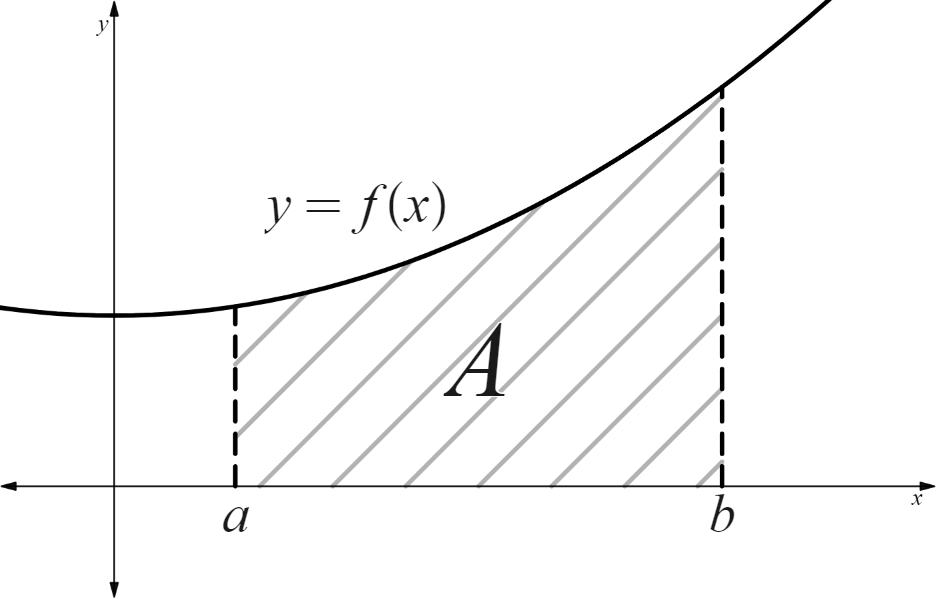
\includegraphics[width=0.9\linewidth]{area_under_a_curve.png}\\
	\end{center}

	\dotfill
	\subsection{Area Between Two Curves}
	Upper function: $f(x)$ or $y_U$\\
	Lower function: $g(x)$ or $y_L$
	\begin{align}
		A=\int_{a}^{b}\left[f(x)-g(x)\right]\,\dd{x}
	\end{align}
	\begin{center}
		or
	\end{center}
	\begin{align}
		A=\int_{a}^{b}\left[y_U-y_L\right]\,\dd{x}
	\end{align}
	\begin{center}
		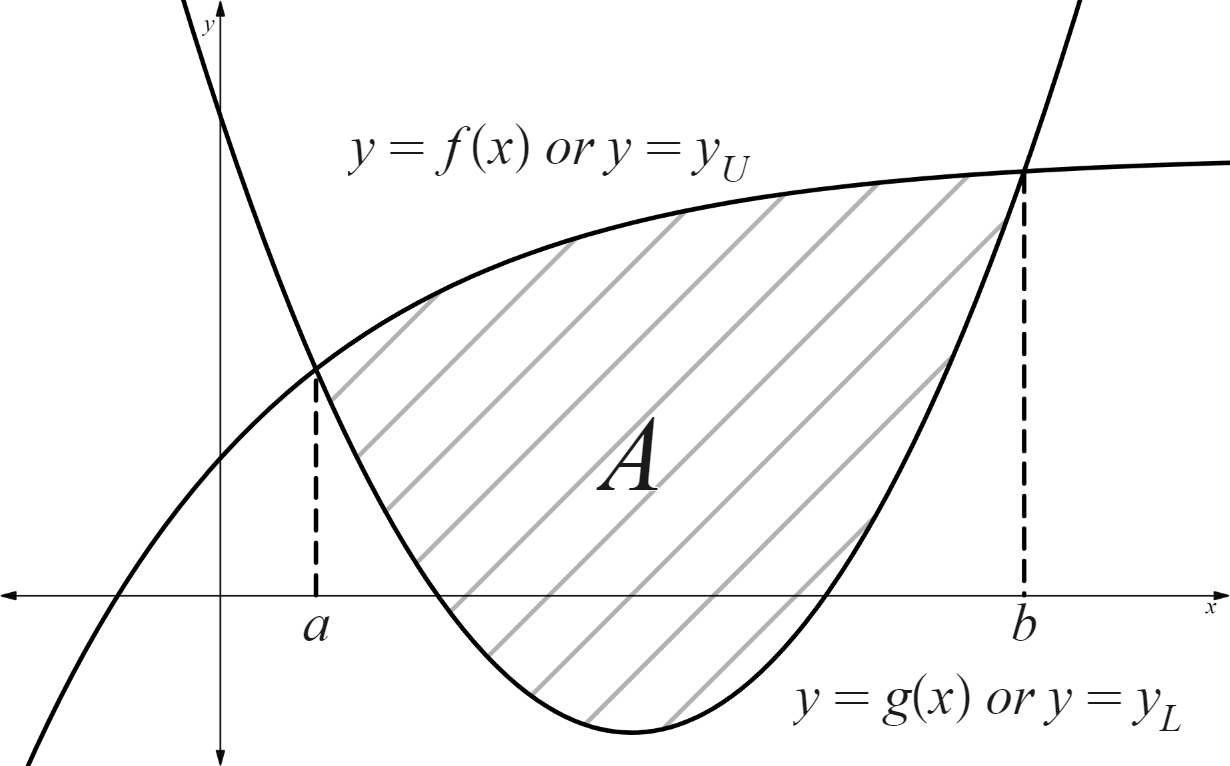
\includegraphics[width=0.9\linewidth]{area_between_two_curves.png}\\
	\end{center}

	\dotfill
	\subsection{Solids of Revolution}
	When the region enclosed by $y=f(x)$, the $x$-axis, $x=a$ and $x=b$ is revolved through $2\pi$ about the $x$-axis, the volume is:
	\begin{align}
		V=\pi\int_{a}^{b}y^2\,\dd{x}
	\end{align}
	When the region enclosed by $y=f(x)$, the $y$-axis, $y=f(a)=c$ and $y=f(b)=d$ is revolved through $2\pi$ about the $y$-axis, the volume is:
	\begin{align}
		V=\pi\int_{c}^{d}x^2\,\dd{y}
	\end{align}

	\dotfill
	\subsection{Volumes for Two Defining Functions}
	Upper function: $f(x)$ or $y_U$\\
	Lower function: $g(x)$ or $y_L$
	\begin{align}
		V=\int_{a}^{b}\left(\left[f(x)\right]^2-\left[g(x)\right]^2\right)\,\dd{x}
	\end{align}
	\begin{center}
		or
	\end{center}
	\begin{align}
		V=\int_{a}^{b}\left(y_U^2-y_L^2\right)\,\dd{x}
	\end{align}

	\hrulefill

	%\pagebreak
	\section{Rates of Change and Differential Equations}
	\subsection{Implicit Differentiation}
	To find $\dv{y}{x}$ for an implicit relationship between $x$ and $y$. A useful property is
	\begin{gather}
		\begin{align}
			\dv{x}\left[x^n\right]=nx^{n-1}
		\end{align}\\
		and\\
		\begin{align}
			\dv{x}\left[y^n\right]=ny^{n-1}\, \dv{y}{x}
		\end{align}
	\end{gather}

	\dotfill
	\subsection{Related Rates}
	Two variables $x$ and $y$ may be related to each other and defined using an equation.
	\begin{align}
		\text{Eg:}\qquad x^2+y^2=5^2
	\end{align}
	The equation can be differentiated in respect to a third parameter $t$ resulting in a related rates equation.
	\begin{align}
		\text{Eg:}\qquad 2x\, \dv{x}{t}+2y\, \dv{y}{t}=0
	\end{align}

	\dotfill
	\subsection{Differential Equations}
	A differential equation is an equation that describes the relationship between a function and its derivatives.

	\dotfill
	\subsection{Differential Equations of the Form $\dv{y}{x}=f(x)$}
	Differential equations of the form $\dv{y}{x}=f(x)$ can be solved using integration.
	\begin{align}
		\dv{y}{x}&=f(x)\\
		\dd{y}&=f(x)\, \dd{x}\\
		\int \dd{y}&=\int f(x)\, \dd{x}\\
		\therefore y&=\int f(x)\, \dd{x}
	\end{align}

	\dotfill
	\subsection{Seperable Differential Equations}
	Differential equations of the form \\$\dv{y}{x}=f(x)g(y)$ can be solved as follows:
	\begin{align}
		\dv{y}{x}&=f(x)g(y)\\
		\frac{1}{g(y)}\, \dd{y}&=f(x)\, \dd{x}\\
		\int \frac{1}{g(y)}\, \dd{y}&=\int f(x)\, \dd{x}
	\end{align}

	\dotfill
	\subsection{Slope Fields}
	For a differential equation $\dv{y}{x}=f(x,y)$, any point $(x,y)$ on the cartesian plane will have a gradient which can be graphically represented using a slope field.

	\dotfill
	\subsection{Logistic Growth}
	Logistic growth is defined by the differential equation
	\begin{align}
		\dv{P}{t}=kP\left(1-\frac{P}{A}\right)
	\end{align}
	The differential equation is solved with partial fractions using the identity:
	\begin{align}
		\frac{A}{P(A-P)}=\frac{1}{P}+\frac{1}{A-P}
	\end{align}
	
	\hrulefill

	\section{Vector Calculus}
	\subsection{Parametric Equations}
	Cartesian equation can be expressed in terms of a parameter such as $t$, defining $x$ and $y$ independently such that $x=x(t)$ and $y=y(t)$.

	\dotfill
	\subsection{Pairs of Uniformly Varying Quantities}
	An object initially at $(x_0,y_0)$ and moving with velocity vector $\vb{v}=\big(\begin{smallmatrix}a \\b \end{smallmatrix}\big)$ has parametric equations
	\begin{align}
		x(t)=x_0+at,\quad y(t)=y_0+bt,\quad t\geq 0
	\end{align}
	The speed of the object is
	\begin{align}
		|\vb{v}|=\sqrt{a^2+b^2}
	\end{align}

	\dotfill
	\subsection{Pairs of Non-Uniformly Varying Quantities}
	%\underline{Velocity}\\
	For the moving object $P(x(t),y(t))$, the velocity vector is:
	\begin{align}
		\vb{v}=\begin{pmatrix}x'(t)\\ y'(t) \end{pmatrix}
	\end{align}
	and the speed is:
	\begin{align}
		\text{speed}=|\vb{v}|=\sqrt{\vb{v}\cdot \vb{v}}=\sqrt{\left[x'(t)\right]^2+\left[y'(t)\right]^2}
	\end{align}
	The gradient of the velocity vector at any point is:
	\begin{align}
		\frac{y'(t)}{x'(t)}=\frac{\left(\dv{y}{t}\right)}{\left(\dv{x}{t}\right)}=\dv{y}{t}\dv{t}{x}=\dv{y}{x}
	\end{align}
	The velocity vector is tangential to the curve, therefore the direction of motion is the gradient.

	\dotfill
	\subsection{B\'ezier Curves}
	Given the starting point $(x_0,y_0)$ and the finishing point $(x_3,y_3)$, and control points $(x_1,y_1)$ and $(x_2,y_2)$, the B\'ezier curve has parametric equations:
	\begin{gather}
		\begin{align}
			&x(t)=a_xt^3+b_xt^2+c_xt+d_x\\
			&y(t)=a_yt^3+b_yt^2+c_yt+d_y,\\
			&0\leq t\leq 1
		\end{align}\\
		where\\
		\begin{cases}
			a_x=x_3-3x_2+3x_1-x_0\\
			b_x=3x_2-6x_1+3x_0\\
			c_x=3x_1-3x_0\\
			d_x=x_0
		\end{cases}\\
		and\\
		\begin{cases}
			a_y=y_3-3y_2+3y_1-y_0\\
			b_y=3y_2-6y_1+3y_0\\
			c_y=3y_1-3y_0\\
			d_y=y_0
		\end{cases}
	\end{gather}
	
	\dotfill
	\subsection{Trigonometric Parameterisation}
	For an object $P$ moving with parametric equations
	\begin{align}
		x(t)=R\cos{\omega t},\quad y(t)=R\sin{\omega t},\quad t\geq 0
	\end{align} 
	where $R>0,\ \omega >0$:
	\begin{itemize}
		\item $R$ controls the radius of the path.
		\item $\omega$ controls the rate of revolutions. The duration of a revolution is $\frac{2\pi}{\omega}$.
		\item The speed of $P$ is $R\omega$.
	\end{itemize}

	\dotfill
	\subsection{Arc Lengths of Parametric Curves}
	The length of the arc traced out by $P(x(t),y(t))$ from time $t=a$ to $t=b$ is:
	\begin{align}
		\int_{a}^{b}|\vb{v}|\,\dd{t}&=\int_{a}^{b}\sqrt{\vb{v}\cdot \vb{v}}\,\dd{t}\\
		&=\int_{a}^{b}\sqrt{\left[x'(t)\right]^2+\left[y'(t)\right]^2}\,\dd{t}
	\end{align}
	\hrulefill

\end{multicols*}
\end{document}